\mysection{エミッタ接地交流増幅回路の設計(原理・計算)}
図\ref{emit_kouryu}にエミッタ接地交流増幅回路を示す。ここでは、どのキャパシタが入力信号を遮断周波数に影響を与えるかを考える。
\begin{figure}[htbp]
  \begin{center}
  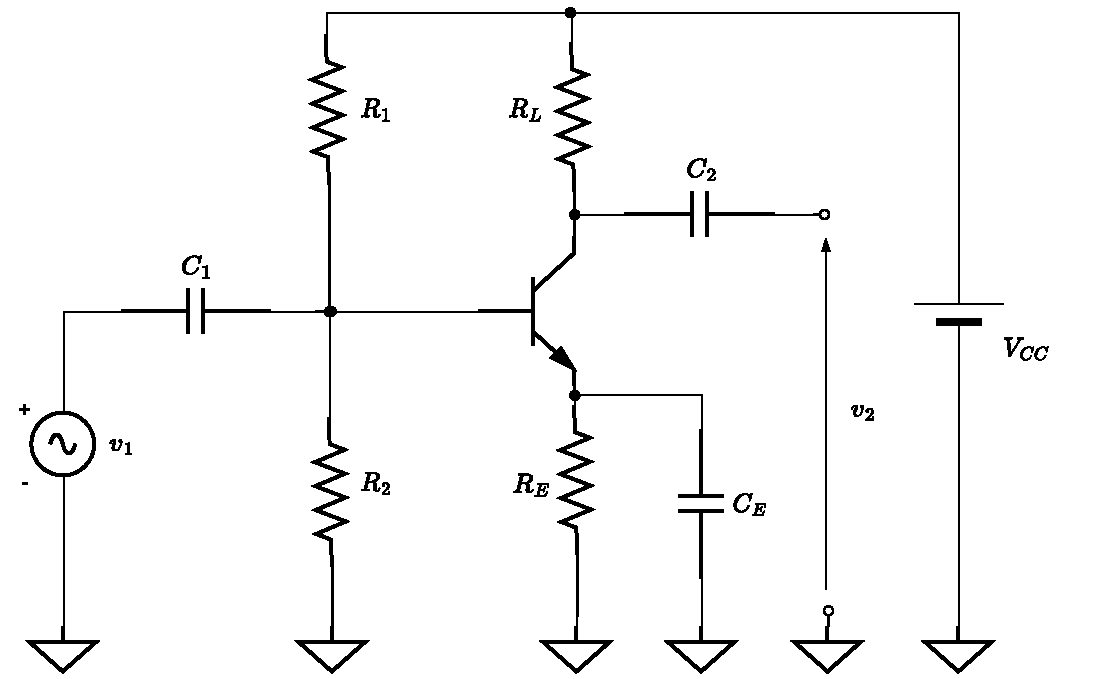
\includegraphics[width=0.68\linewidth]{img/45.pdf}
  \caption{エミッタ接地交流増幅回路}
  \label{emit_kouryu}
  \end{center}
\end{figure}

$C_{E}$: バイパスキャパシタ\\
$C_{1}, C_{2}$: 結合キャパシタ(直流信号を遮断して交流信号だけを通過)

\mysubsection{等価回路}
エミッタ接地微小信号等価回路と微小信号の変化分を表す特性を図に示す。
微小信号とは、小さな振幅の交流信号のことである。
$r_e$ は、ベース - エミッタ間の pn 接合ダイオードを抵抗に置き換えたものである。
直流に対しては、この pn 接合はダイオードと考えられるが、ベースの入力信号が微小変化する場合には、$V_{BE}$ の変化に対してエミッタ電流 $I_E$ の変化が比例して変化するものと考えられる。
\begin{figure}[htb]
  \begin{center}
  \subfigure[エミッタ接地微小信号等価回路]{
  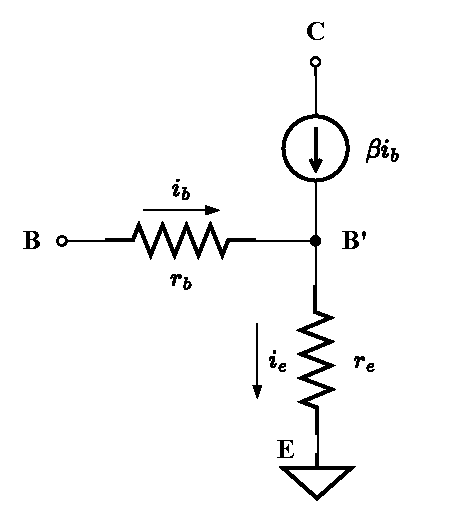
\includegraphics[width=.45\columnwidth]{img/46.pdf}
  }
  \subfigure[微小信号の変化分を表す特性($V_{BE}$-$I_E$特性の再喝)]{
  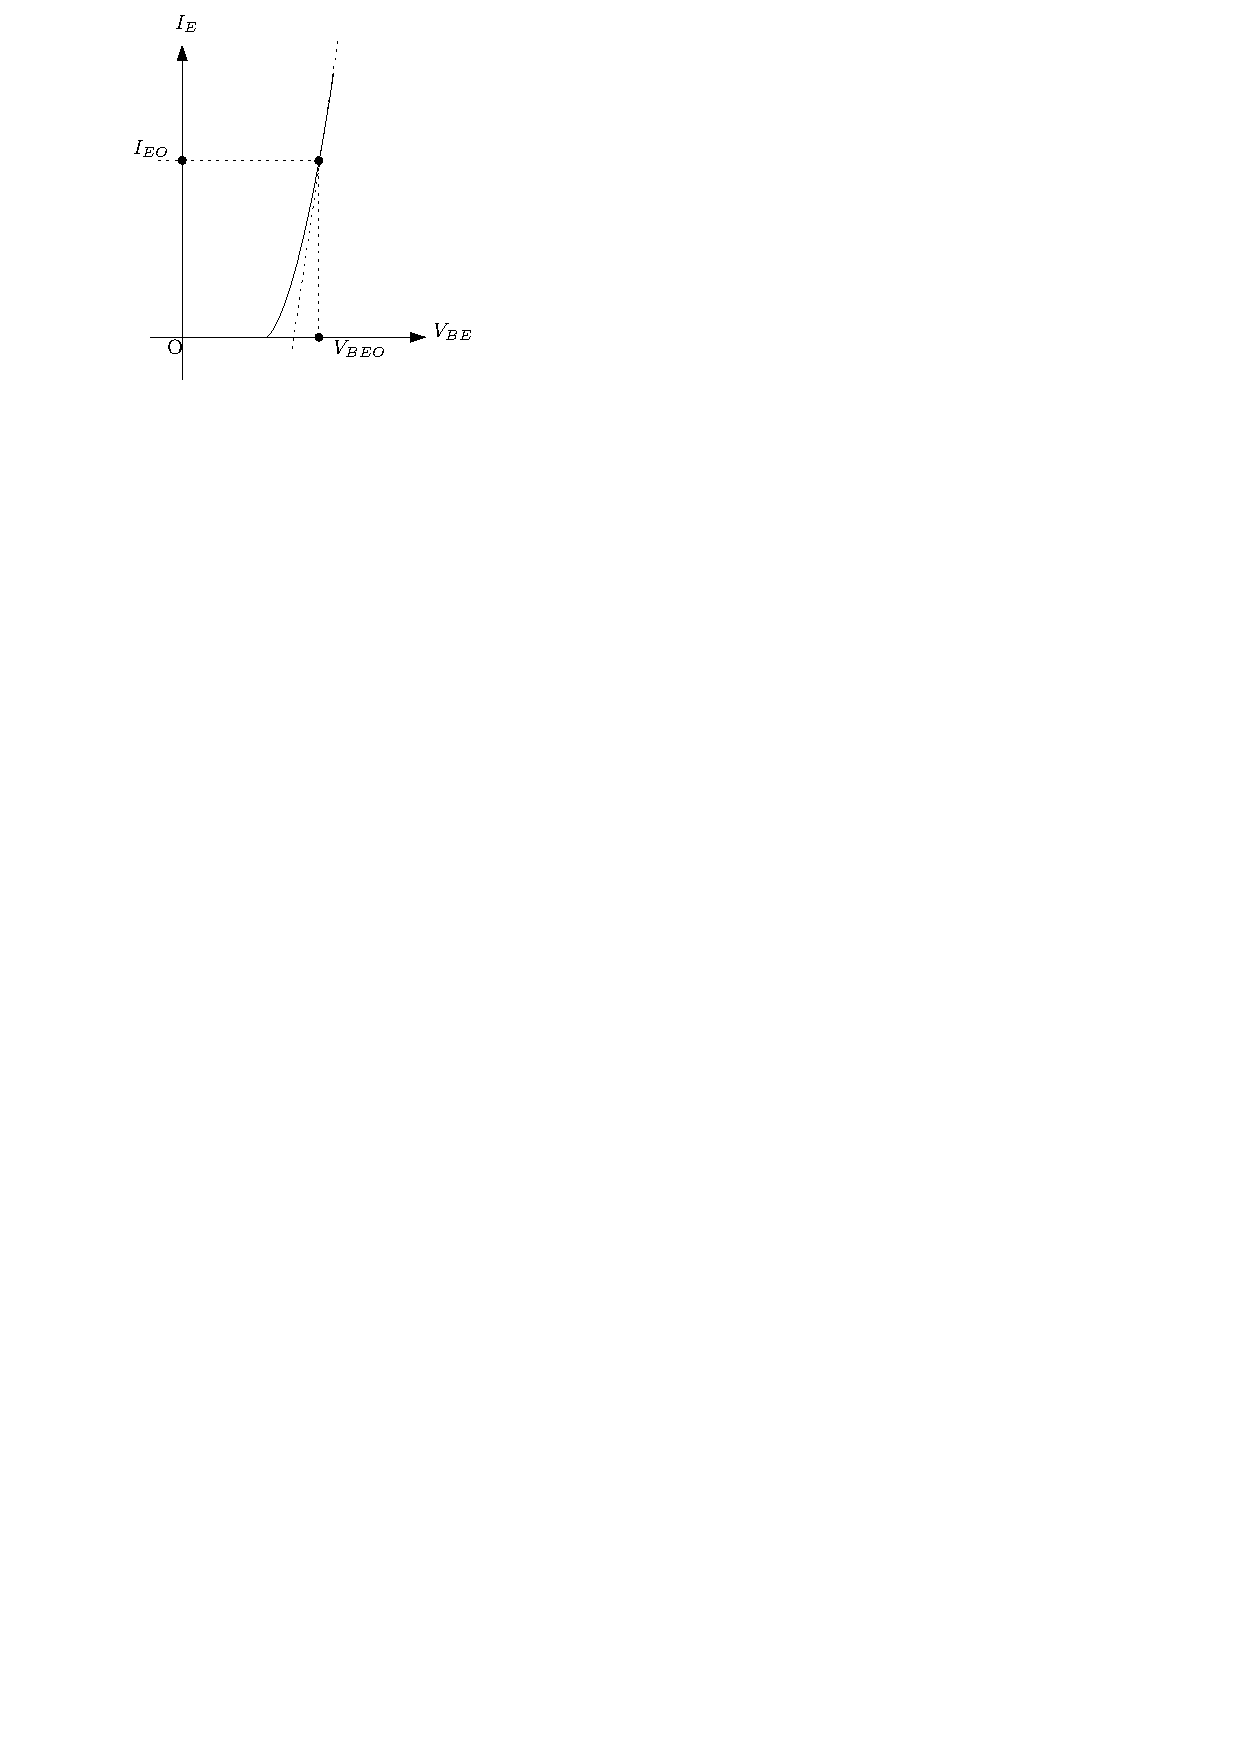
\includegraphics[width=.45\columnwidth]{img/47.pdf}
  }
  \caption{微小信号等価回路の原理}
  \label{vbe_ie}
  \end{center}
\end{figure}

$I_E \approx I_S \exp(\frac{q}{kT}V_{BE})$ を $V_{BE}$ で微分すると(これが、$I_E$-$V_{BE}$曲線の傾きとなる。)\\
\begin{align}
  & \frac{1}{r_e} = \frac{dI_E}{dV_{BE}} \approx \frac{q}{kT}I_S\exp(\frac{q}{kT}V_{BE}) = \frac{q}{kT}I_E\\
  & r_e = \frac{kT}{q}\cdot\frac{1}{I_{EO}} \approx \frac{0.026}{I_{EO}}
\end{align}

\mysubsection{電圧増幅度の計算}
図\ref{emit_touka}に、微小信号等価回路を利用して描いたエミッタ接地交流等価回路を示す。

\begin{figure}[htbp]
  \begin{center}
  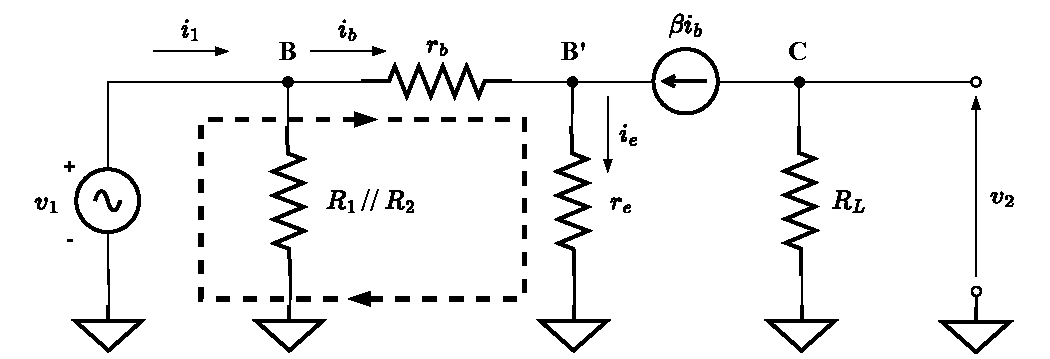
\includegraphics[width=0.8\linewidth]{img/48.pdf}
  \caption{エミッタ接地交流増幅回路の等価回路}
  \label{emit_touka}
  \end{center}
\end{figure}

\begin{description}
  \item [入力インピーダンス]: $R_1//R_2$と$Z_i$が並列に接続されている。\\
  ($Z_i$は、ベース端子から見た入力インピーダンス)
  ここで、$Z_i = v_1/i_b$より、点線のループに沿ってキルヒホッフの法則を適用すると、
  \begin{align}
    v_1 = r_bi_b+r_ei_e \label{eq1}
  \end{align}
  B'点にキルヒホッフの電流則を適用すると、
  \begin{align}
    i_e = (1+\beta)i_b \label{eq2}
  \end{align}
  式\eqref{eq1}、\eqref{eq2}より、$i_e$ を消去して、
  \begin{align}
    v_1 = r_bi_b+r_e(1+\beta)i_b
  \end{align}
よってベースから見た入力インピーダンス $Z_i$ は、
  \begin{align}
    Z_i = \frac{v_1}{i_b} = r_b+(1+\beta)r_e
  \end{align}
$Z_i$ を用いると、エミッタ接地回路の入力端子から見たインピーダンス $Z_{in}$ は、
  \begin{align}
    Z_{in} = R_1//R_2//Z_i
  \end{align}
となる。
  \item [電圧増幅度]: 負荷抵抗 $R_L$ には下から上に流れる電流 $\beta i_b$ が流れている。\\
  よって、出力電圧 $v_2$ は、逆の極性を持つため、
  \begin{align}
    & v_2 = - R_L\beta i_b\\
    & i_b = \frac{v_1}{r_b+(1+\beta)r_e}\\
    & A_v = \frac{v_2}{v_1} = \frac{-\beta R_L}{r_b+(1+\beta)r_e} = \frac{-\beta R_L}{Z_i}    
  \end{align}

\end{description}

\mysubsection{$C_1$ による遮断周波数 $f_{C1}$}
  入力側の結合キャパシタ $C_1$を考慮した入力部の等価回路を図\ref{C1}に示す。

  \begin{figure}[htbp]
    \begin{center}
    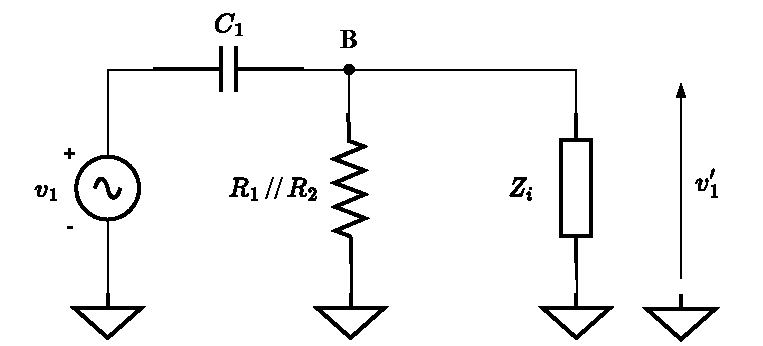
\includegraphics[width=0.8\linewidth]{img/49.pdf}
    \caption{$C_1$を考慮したエミッタ接地交流増幅回路の等価回路}
    \label{C1}
    \end{center}
  \end{figure}
  $v_1'$: ベースへの交流入力電圧 $v_1$: 元の入力信号として、\\
  電圧 $v_1$$v_1'$との比を求めると、
  \begin{align}
    & \frac{v_1'}{v_1} = \frac{R_1//R_2//Z_i}{\frac{1}{j\omega C_1}+R_1//R_2//Z_i} = \frac{1}{1+\frac{1}{j\omega C_1(R_1//R_2//Z_i)}}\\
    & Z_i = \frac{v_1}{i_b} = r_b+(1+\beta)r_e    
  \end{align}

  キャパシタ $C_1$ を入れた時の電圧増幅度 $A'_v = \frac{v_2}{v_1}$ は、$A_v = \frac{v_2}{v'_1}$ として、
  \begin{align}
    A'_v = \frac{v_2}{v_1} = \frac{v'_1}{v_1}\cdot\frac{v_2}{v'_1} = A_v\frac{v'_1}{v_1} = \frac{-\beta R_L}{Z_i} \cdot \frac{1}{1+\frac{1}{j\omega C_1(R_1//R_2//Z_i)}}    
  \end{align}

  $A'_v$ の絶対値、(振幅伝達関数)は、
  \begin{align}
    |A'_v| = \frac{\beta R_L}{Z_i} \times \frac{1}{\sqrt{1+(\frac{1}{\omega C_1(R_1//R_2//Z_i})^2}}
  \end{align}
  となる。
  $\frac{\beta R_L}{Z_i}$は、全てのキャパシタを短絡して考えた $A_v$ の式と同じである。
  この増幅度から、$\frac{1}{\sqrt{2}}$ に低下する周波数(低域遮断周波数$f_{C1}$)は、
  $\omega C_1(R_1//R_2//Z_i) = 1$より、
  \begin{align}
    & 2\pi f_{C1}C_1(R_1 // R_2 // Z_i) = 1\\
    & C_1 = \frac{1}{2\pi f_{C1} (R_1//R_2//Z_i)} = 1    
  \end{align}


\mysubsection{$C_2$による遮断周波数$f_{C2}$}
入力側の結合キャパシタ$C_2$を入れた入力部の等価回路を図\ref{c2}に示す。
\begin{figure}[htbp]
  \begin{center}
  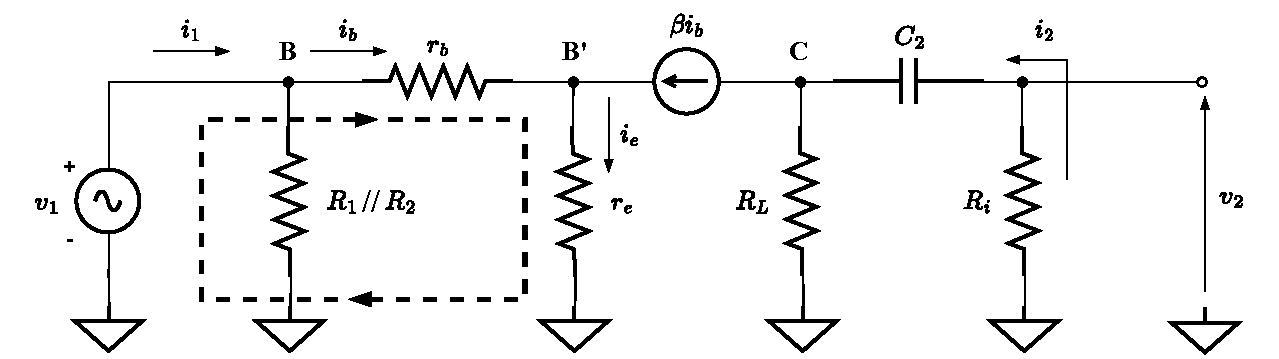
\includegraphics[width=0.8\linewidth]{img/50.pdf}
  \caption{$C_2$を考慮したエミッタ接地交流増幅回路の等価回路}
  \label{c2}
  \end{center}
\end{figure}
図の点線に沿ってキルヒホッフの電圧則を適用すると、
\begin{align}
  v_1 = r_bi_b+(1+\beta)r_ei_b  
\end{align}

出力側に流れる電流$i_2$を電流源$\beta i_b$から求めると、出力側の回路は$R_L$と、直列の$C_2-R_i$が並列接続された形であるため、\\
\begin{align}
  i_2 = \beta i_b \times \frac{R_L}{R_L+(\frac{1}{j\omega C_2}+R_i)}
\end{align}
で求まる。また、出力側電圧$v_2$は、
\begin{align}
  v_2 = - i_2R_i
\end{align}
よって、電圧増幅度$A_v$は、
\begin{align}
\begin{aligned}
  A_v & = \frac{v_2}{v_1} = \frac{-i_2R_i}{r_bi_b+(1+\beta)r_ei_b} = \frac{\frac{-\beta R_LR_i}{R_L+(\frac{1}{j\omega C_2}+R_i)}}{r_b+(1+\beta)r_e}\\
  & = \frac{-\beta}{r_bi_b+(1+\beta)r_ei_b} \cdot \frac{R_LR_i}{R_L+(\frac{1}{j\omega C_2}+R_i)} = \frac{-\beta}{r_bi_b+(1+\beta)r_ei_b} \cdot \frac{\frac{R_LR_i}{R_L+R_i}}{1+\frac{1}{j\omega C_2(R_L+R_i)}}\\
  & = \frac{-\beta R'_L}{r_bi_b+(1+\beta)r_ei_b} \cdot \frac{1}{1+\frac{1}{j\omega C_2(R_L+R_i)}}
\end{aligned}
\end{align}
と求まる。($R'_L = R_L//R_i$)\\
$\frac{-\beta R'_L}{Z_i} \cdot \frac{1}{1+\frac{1}{j\omega C_2(R_L+R_i)}}$ と、$-\frac{\beta R_L}{Z_i}$ と見比べると、$C_2$ を短絡して考えられる 周蓮での増幅度に相当する。つまり、$R_L$ と次段の入力インピーダンス $R_i$ が並列接続された形で増幅度が決まる。
\begin{align}
  |A_v| = \frac{\beta R'_L}{Z_i} \cdot \frac{1}{\sqrt{1+(\frac{1}{(\omega C_2(R_L+R_i)})^2}}  
\end{align}

$C_2$ を短絡して考えた場合の値 $\frac{\beta R'_L}{Z_i}$ に対して、増幅度が $1/sqrt{2}$ となる周波数(低域遮断周波数 $f_{C2}$)は、$\omega C_2(R_L+R_i) = 1$、$2\pi f_{C2} C_2(R_L+R_i) = 1$ より、
\begin{align}
  f_{C2} = \frac{1}{2\pi C_2(R_L+R_i)}  
\end{align}

\mysubsection{$C_E$による遮断周波数 $f_{CE}$}
抵抗 $R_E$ に並列にバイパスキャパシタ$C_E$を入れた等価回路を図\ref{ce}に示す。
\begin{figure}[htbp]
  \begin{center}
  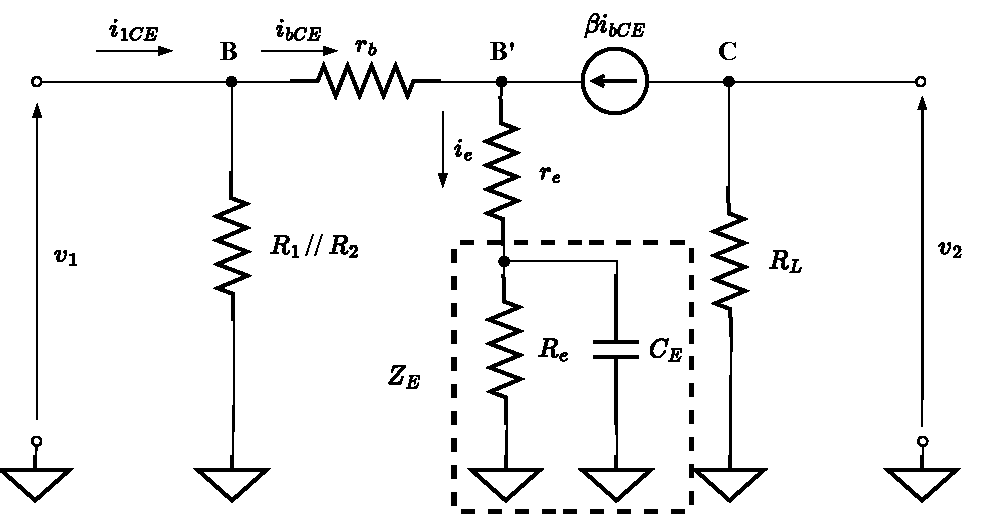
\includegraphics[width=0.8\linewidth]{img/51.pdf}
  \caption{$C_E$を考慮したエミッタ接地交流増幅回路の等価回路}
  \label{ce}
  \end{center}
\end{figure}

$C_E, R_E$ の並列インピーダンス $Z_E$は、
\begin{align}
  Z_E = \frac{R_E \cdot \frac{1}{j\omega C_E}}{R_E+\frac{1}{j\omega C_E}} = \frac{R_E}{1+j\omega C_ER_E} \label{ze}
\end{align}

$C_E$ が短絡している場合、$Z_E = 0$ となる。$v_1 \rightarrow r_b \rightarrow r_e$のループにキルヒホッフの電圧則を適用した式 $v_1 = r_bi_{bCE}+r_e(1+\beta)i_{bCE}$ を用いて、
\begin{align}
  Z_i = \frac{v_1}{i_{bCE}} = r_b+(1+\beta)r_e
\end{align}
となる。($Z_i$ベース端子B から見たトランジスタの入力インピーダンス)

$r_b: 50 ~ 500 \Omega$ 程度 $\beta$: 100 ~ 500 程度 ダイオードの交流等価回路 $r_e$: 数10 $\Omega$ $(1+\beta)r_e >> r_b, \beta >> 1$ として、
\begin{align}
  Z_i \approx (1+\beta)r_e \approx \beta r_e \label{zi}
\end{align}
となる。

電圧増幅度 $A_v = \frac{v_2}{v_1}$ について、$v_1 \rightarrow r_b \rightarrow r_e \rightarrow Z_E$ のループにキルヒホッフの電圧則を適用すると

$v_1 = r_b i_{bCE}+(r_e+Z_E)(1+\beta)i_{bCE}$
$= [r_b+(1+\beta)(r_e+Z_E)]i_{bCE} = [r_b+(1+\beta)r_e+(1+\beta)Z_E]i_{bCE}$
$= [Z_i+(1+\beta)Z_E]i_{bCE}$ となる。
$v_2 = -R_L\beta i_{bCE}$ ($v_2$ は、電流$\beta i_{bCE}$ が負荷抵抗 $R_L$ を下から上に流れる。)

\begin{align}
  A_v = \frac{v_2}{v_1} =\frac{-\beta R_L}{Z_i+(1+\beta)Z_E} \label{av}  
\end{align}

式\eqref{av}を図\eqref{ze}、図\eqref{zi}に代入して、
\begin{align}
  \begin{aligned}
  A_v & = \frac{-\beta R_L}{Z_i+(1+\beta)Z_E} \approx \frac{-\beta R_L}{Z_i+\beta \frac{R_E}{1+j\omega C_E R_E}}\\
  & = \frac{-\beta R_L(1+j\omega C_E R_E)}{Z_i(1+j\omega C_ER_E)+\beta R_E} = -\beta R_L \cdot \frac{1+j\omega C_E R_E}{Z_i+\beta R_E+j\omega C_ER_EZ_i} \approx -\beta R_L \cdot \frac{1+j\omega C_E R_E}{\beta r_e+\beta R_E + j\omega C_E R_E Z_i}\\
  & = -\beta R_L R_E \cdot \frac{1+j\omega C_ER_E}{\beta(r_e+R_E)+j\omega C_E R_E Z_i} \approx -\beta R_L \cdot \frac{1+j\omega C_E R_E}{\beta R_E + j\omega C_E R_E Z_i}\\
  & = -\frac{\beta R_L}{R_E} \cdot \frac{1+j\omega C_E R_E}{\beta + j\omega C_E Z_i} = -\frac{R_L}{R_E} \cdot \frac{1+j\omega C_E R_E}{1+j\omega C_E Z_i/\beta} \\ \label{}
  \end{aligned}
\end{align}
式\eqref{zi}より、
\begin{align}
  A_v \approx -\frac{R_L}{R_E}\cdot\frac{1+j\omega C_ER_E}{1+j\omega C_EZ_i/\beta} \approx -\frac{R_L}{R_E}\cdot \frac{1+j\omega C_E R_E}{1+j\omega C_E r_e}
\end{align}
$f \to \infty, \omega \to \infty$ の場合、\\
$\left.A_v\right|_{\omega \to 0} \approx -\frac{R_L}{R_E}$ と一定値(低域の電圧増幅度) になり、\\
$\left.A_v\right|_{\omega \to \infty} \approx -\frac{R_L}{r_e} \leftarrow$ ロピタルの定理\\
と、一定値(中域での電圧増幅度)となる。

$-\frac{R_L}{R_E} \cdot \frac{1+j\omega C_E R_E}{1+j\omega C_E r_e}$ の分母分子に関係する特徴的な周波数について

\begin{align}
  f_{CE1} = \frac{1}{2\pi C_E Z_i/\beta} \approx \frac{1}{2\pi C_E r_e}\\
  f_{CE2} = \frac{1}{2\pi C_E R_E}\\
  A_v \approx -\frac{R_L}{R_E} \cdot \frac{1+j(f/f_{CE2})}{1+j(f/f_{CE1})}\\
  A_v \approx -\frac{R_L}{R_E} \cdot \frac{1+j(f/f_{CE2})}{1+j(f/f_{CE1})}\\
  |A_v| \approx \frac{R_L}{R_E} \cdot \sqrt{\frac{1+(f/f_{CE2})^2}{1+(f/f_{CE1})^2}}
\end{align}

この式は、低周波数側から周波数を増加させるとき、$f_{CE2}, f_{CE1}$ で2回折れ曲がる形の関数である。

$f_{CE2}$ は、$C_E R_E$ で決まる周波数
低周波数 → 高周波数に増加するときに増幅度が上りはじめる周波数

$f_{CE1}$ は、時定数 $C_E r_e$ で決まる周波数で、高周波 → 低周波数に減少するときに
増幅度が下がりはじめる周波数である。したがって、バイパスキャパシタ $C_E$ を含む図の等価回路では、低域遮断周波数は、$f_{CE1}$ となる。

\mysubsection{低域遮断周波数のまとめ}
入力側キャパシタ $C_1$: $f_{C1} = \frac{1}{2\pi C_1(R_1//R_2//Z_i)}$\\
出力側キャパシタ $C_2$: $f_{C2} = \frac{1}{2\pi C_2(R_L+R_i)}$\\
バイパスキャパシタ $C_E$: $f_{CE1} = \frac{1}{2\pi C_E Z_i/\beta} \approx \frac{1}{2\pi C_E r_e}$\\

$R_1, R_2, R_L, R_i, Z_i$ が、k$\Omega$ オーダに対し、$r_e \approx \frac{Z_i}{\beta}$ は、\\
1 ~ 10 $\Omega$ オーダ各キャパシタの静電容量を同じにすると、$C_E$ による周波数 $f_{CE1}$ が最も大きな値となる。つまり、低域遮断周波数は、トランジスタの交流増幅率の低下、ベース- コレクタ間容量によるベース端子への逆位相信号入力(負帰還)、回路を組み立てる配線の分布容量など複数の要因がからみ合っており、高域遮断周波数の設計には、より高度な回路に関する知見が必要である。

\mysubsection{諸量計算$r_e$、$A_v$、低域遮断周波数}
$r_e, A_v(電圧増幅度), 低域遮断周波数 f_{CE1}, f_{C1}, f_{C2}$\\
条件1 $C_1, C_2$は、$100 \mu$F を使う
\begin{enumerate}
  \setlength{\parskip}{0cm} % 段落間
  \setlength{\itemsep}{0cm} % 項目間
  \item $r_e \approx \frac{kT}{q} \cdot \frac{1}{I_{EQ}}$
  $r_e \approx \frac{0.026}{I_{EO}} (I_{EO} \approx I_{CO}) (\frac{kT}{q} は定数)$
  \item $A_v = \frac{v_2}{v_1} = -\frac{\beta R_L}{Z_i} = -\frac{R_L}{Z_i/\beta} \approx -\frac{R_L}{r_e} = \frac{506}{3.3} \approx -153$
\end{enumerate}

条件2: 低域遮断周波数$f_{CE1} = 20$ Hz として設計)
$$f_{CE1} \approx \frac{1}{2\pi C_E r_e} \Rightarrow C_E \approx \frac{1}{2\pi f_{CE1}r_e}$$


\mysection{エミッタ接地交流増幅回路の設計手順}
\begin{enumerate}
  \setlength{\parskip}{0cm}
  \setlength{\itemsep}{0cm}
  \item $r_e \approx \frac{0.026}{I_{EO}} \approx \frac{0.026}{I_{CO}} = \frac{26\times10^{-3}}{5.5 \times 10^{-3}} \approx 4.7272 [\Omega]$
  \item $A_v = \frac{v_2}{v_1} = -\frac{\beta R_L}{Z_i} = -\frac{R_L}{Z_i/\beta} \approx -\frac{818.18}{4.72} = -173.3432...$
  \item $C_E$: 低域遮断周波数を 20 Hz として設定(可聴周波数の下限)
  \begin{align}
    f_{CE1} \approx \frac{1}{2\pi C_Er_e} \Rightarrow C_E \approx \frac{1}{2\pi f_{CE1} r_e} \approx \frac{1}{2\pi \times 20 \times 4.72} = 1.68596 \times 10^{-3} = 1686 \mu\textrm{F}
  \end{align}
\end{enumerate}
$C_1, C_2は、100 \mu\textrm{F} より、次段の入力インピーダンスを R_i = 1\textrm{k}\Omega と仮定$

\begin{align}
  & f_{C1} = \frac{1}{2\pi C_1(R_1//R_2//Z_i)} \approx \frac{10^4}{2\pi \times (15.2\times10^3//3.4\times10^3//10^3)} \approx \frac{10^4}{2\pi \times 735.344} \approx 2.1643\textrm{Hz}\\
  & f_{C2} = \frac{1}{2\pi C_2(R_L+R_i)} \approx \frac{1}{2\pi \times 10^{-4} \times 1.818 \times 10^3} = 0.8754[\textrm{Hz}]  
\end{align}

$f_{C1}, f_{C2}$は、20 Hz と比べてかなり小さい。